\documentclass[a4paper]{article}
\usepackage{geometry}
\usepackage{graphicx}
\usepackage{natbib}
\usepackage{amsmath}
\usepackage{amssymb}
\usepackage{amsthm}
\usepackage{paralist}
\usepackage{epstopdf}
\usepackage{tabularx}
\usepackage{longtable}
\usepackage{multirow}
\usepackage{multicol}
\usepackage[hidelinks]{hyperref}
\usepackage{fancyvrb}
\usepackage{float}
\usepackage{paralist}
\usepackage[svgname]{xcolor}
\usepackage{enumerate}
\usepackage{array}
\usepackage{times}
\usepackage{url}
\usepackage{fancyhdr}
\usepackage{comment}
\usepackage{environ}
\usepackage{times}
\usepackage{textcomp}
\usepackage{caption}
\usepackage{bbm}
\usepackage{enumitem}
\usepackage{algorithm}
\usepackage{algpseudocode}
\usepackage{caption}
\usepackage{subcaption}


\urlstyle{rm}

\setlength\parindent{0pt} % Removes all indentation from paragraphs
\theoremstyle{definition}
\newtheorem{definition}{Definition}[]
\newtheorem{conjecture}{Conjecture}[]
\newtheorem{example}{Example}[]
\newtheorem{theorem}{Theorem}[]
\newtheorem{lemma}{Lemma}
\newtheorem{proposition}{Proposition}
\newtheorem{corollary}{Corollary}

\floatname{algorithm}{Procedure}
\renewcommand{\algorithmicrequire}{\textbf{Input:}}
\renewcommand{\algorithmicensure}{\textbf{Output:}}
\newcommand{\abs}[1]{\lvert#1\rvert}
\newcommand{\norm}[1]{\lVert#1\rVert}
\newcommand{\RR}{\mathbb{R}}
\newcommand{\CC}{\mathbb{C}}
\newcommand{\Nat}{\mathbb{N}}
\newcommand{\br}[1]{\{#1\}}
\DeclareMathOperator*{\argmin}{arg\,min}
\DeclareMathOperator*{\argmax}{arg\,max}
\renewcommand{\qedsymbol}{$\blacksquare$}

\definecolor{dkgreen}{rgb}{0,0.6,0}
\definecolor{gray}{rgb}{0.5,0.5,0.5}
\definecolor{mauve}{rgb}{0.58,0,0.82}

\newcommand{\Var}{\mathrm{Var}}
\newcommand{\Cov}{\mathrm{Cov}}

\newcommand{\vc}[1]{\boldsymbol{#1}}
\newcommand{\xv}{\vc{x}}
\newcommand{\Sigmav}{\vc{\Sigma}}
\newcommand{\alphav}{\vc{\alpha}}
\newcommand{\muv}{\vc{\mu}}

\newcommand{\red}[1]{\textcolor{red}{#1}}

\def\x{\mathbf x}
\def\y{\mathbf y}
\def\w{\mathbf w}
\def\v{\mathbf v}
\def\E{\mathbb E}
\def\V{\mathbb V}
\def\ind{\mathbbm 1}

% TO SHOW SOLUTIONS, include following (else comment out):
\newenvironment{soln}{
	\leavevmode\color{blue}\ignorespaces
}{}

\hypersetup{
	%    colorlinks,
	linkcolor={red!50!black},
	citecolor={blue!50!black},
	urlcolor={blue!80!black}
}

\geometry{
	top=1in,            % <-- you want to adjust this
	inner=1in,
	outer=1in,
	bottom=1in,
	headheight=3em,       % <-- and this
	headsep=2em,          % <-- and this
	footskip=3em,
}


\pagestyle{fancyplain}
\lhead{\fancyplain{}{Homework 6}}
\rhead{\fancyplain{}{CS 760 Machine Learning}}
\cfoot{\thepage}

\title{\textsc{Homework 6}} % Title

%%% NOTE:  Replace 'NAME HERE' etc., and delete any "\red{}" wrappers (so it won't show up as red)

\author{Dario Placencio - 907 284 6018}

\date{}

\begin{document}
	
	\maketitle 
	
        \textbf{Instructions:}
        Use this latex file as a template to develop your homework. Submit your homework on time as a single pdf file. Please wrap your code and upload to a public GitHub repo, then attach the link below the instructions so that we can access it. Answers to the questions that are not within the pdf are not accepted. This includes external links or answers attached to the code implementation. Late submissions may not be accepted. You can choose any programming language (i.e. python, R, or MATLAB). Please check Piazza for updates about the homework. It is ok to share the results of the experiments and compare them with each other.
        \vspace{0.1in}
	
	\section{Implementation: GAN (50 pts)}
	In this part, you are expected to implement GAN with MNIST dataset. We have provided a base jupyter notebook (gan-base.ipynb) for you to start with, which provides a model setup and training configurations to train GAN with MNIST dataset.
	
	\begin{enumerate} [label=(\alph*)]
		\item Implement training loop and report learning curves and generated images in epoch 1, 50, 100. Note that drawing learning curves and visualization of images are already implemented in provided jupyter notebook. \hfill (20 pts)
		
		\begin{algorithm}
			\caption{Training GAN, modified from \cite{goodfellow2014generative}}\label{alg:GAN}
			\begin{algorithmic}
				\Require $m$: real data batch size, $n_{z}$: fake data batch size
				\Ensure Discriminator $D$, Generator $G$
				
				\For{number of training iterations}
				
				\State{$\#$ Training discriminator}
				\State{Sample minibatch of $n_{z}$ noise samples $\{z^{(1)}, z^{(2)}, \cdots, z^{(n_{z})}\}$ from noise prior $p_{g}(z)$}
				\State{Sample minibatch of $\{x^{(1)}, x^{(2)}, \cdots, x^{(m)}\}$}
				\State{Update the discriminator by ascending its stochastic  gradient:
					$$\nabla_{\theta_{d}} \big ( \cfrac{1}{m}  \sum_{i=1}^{m}  \log D(x^{(i)})  + \cfrac{1}{n_{z}} \sum_{i=1}^{n_{z}}  \log (1-D(G(z^{(i)})))\big )$$
				}
				
				\State{$\#$ Training generator}
				\State{Sample minibatch of $n_{z}$ noise samples $\{z^{(1)}, z^{(2)}, \cdots, z^{(n_{z})}\}$ from noise prior $p_{g}(z)$}
				\State{Update the generator  by ascending its stochastic  gradient:
					$$\nabla_{\theta_{g}}  \cfrac{1}{n_{z}} \sum_{i=1}^{n_{z}}  \log D(G(z^{(i)}))\big )$$
				}
				\EndFor
				
				\State{$\#$ The gradient-based updates can use any standard gradient-based learning rule. In the base code, we are using Adam optimizer \citep{kingma2014adam}}
			\end{algorithmic}
		\end{algorithm}
		
		Expected results are as follows.
		
		\begin{figure}[H]
			\centering
			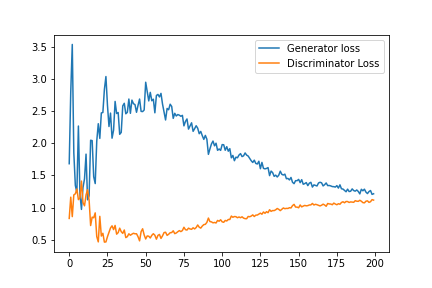
\includegraphics[width=0.7\textwidth]{gan_q1_loss.png}
			\caption{Learning curve}
			\label{fig:gan_q1_loss}
		\end{figure}
		
		\begin{figure}[H]
			\centering
			\begin{subfigure}[b]{0.3\textwidth}
				\centering
				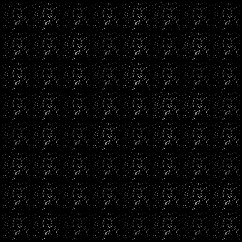
\includegraphics[width=\textwidth]{gan_q1_epoch1.png}
				\caption{epoch 1}
			\end{subfigure}
			\hfill
			\begin{subfigure}[b]{0.3\textwidth}
				\centering
				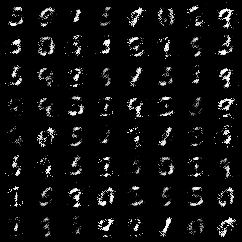
\includegraphics[width=\textwidth]{gan_q1_epoch50.png}
				\caption{epoch 50}
			\end{subfigure}
			\hfill
			\begin{subfigure}[b]{0.3\textwidth}
				\centering
				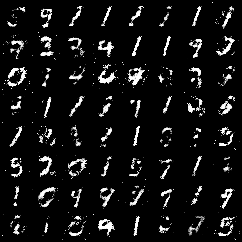
\includegraphics[width=\textwidth]{gan_q1_epoch100.png}
				\caption{epoch 100}
			\end{subfigure}
			\caption{Generated images by $G$}
			\label{fig:three graphs}
		\end{figure}
		
		
		\begin{soln}
		These are the results of executing the first GAN, code attached below.
		\begin{figure}[H]
			\centering
			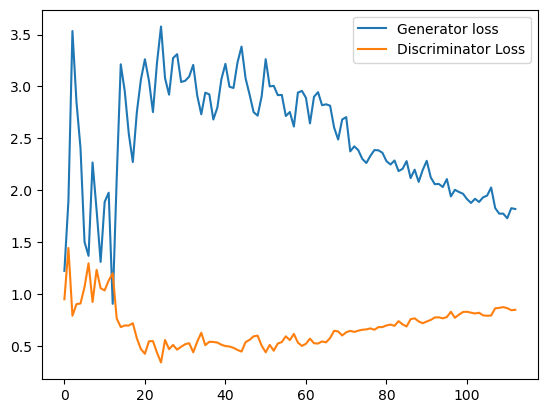
\includegraphics[width=0.7\textwidth]{1-LearningCurve.png}
			\caption{Learning curve for GAN (a)}
			\label{fig:loss_1}
		\end{figure}
		
		\begin{figure}[H]
			\centering
			\begin{subfigure}[b]{0.3\textwidth}
				\centering
				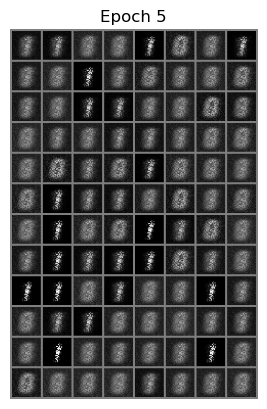
\includegraphics[width=\textwidth]{1-Epoch5.png}
				\caption{epoch 5}
			\end{subfigure}
			\hfill
			\begin{subfigure}[b]{0.3\textwidth}
				\centering
				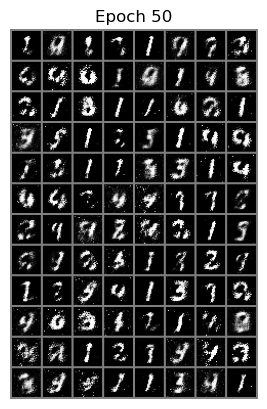
\includegraphics[width=\textwidth]{1-Epoch50.png}
				\caption{epoch 50}
			\end{subfigure}
			\hfill
			\begin{subfigure}[b]{0.3\textwidth}
				\centering
				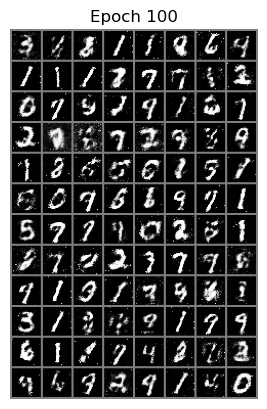
\includegraphics[width=\textwidth]{1-Epoch100.png}
				\caption{epoch 100}
			\end{subfigure}
			\caption{Epochs for GAN (a)}
			\label{epochs_1}
		\end{figure}
		\end{soln}

		\item Replace the generator update rule as the original one in the slide,\\
		``Update the generator by descending its stochastic gradient:
		
		$$\nabla_{\theta_{g}}  \cfrac{1}{n_{z}}  \sum_{i=1}^{n_{z}}\log (1-D(G(z^{(i)})))\big )$$
		"
		, and report learning curves and generated images in epoch 1, 50, 100. Compare the result with (a). Note that it may not work. If training does not work, explain why it doesn't work. \\
        You may find this helpful: https://jonathan-hui.medium.com/gan-what-is-wrong-with-the-gan-cost-function-6f594162ce01
		\hfill (10 pts)
		
		\begin{soln}
			These are the results of executing the second GAN, code attached below.
			\begin{figure}[H]
				\centering
				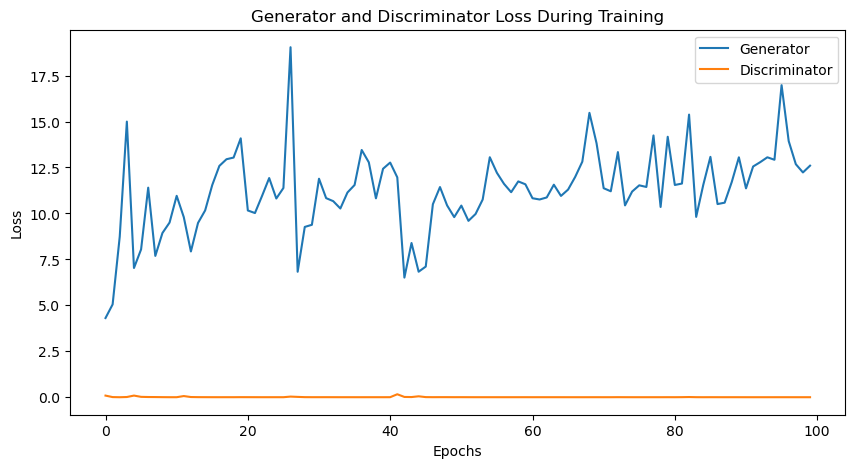
\includegraphics[width=0.7\textwidth]{2-LearningCurve.png}
				\caption{Learning curve for GAN (b)}
				\label{fig:loss_2}
			\end{figure}
			
			\begin{figure}[H]
				\centering
				\begin{subfigure}[b]{0.3\textwidth}
					\centering
					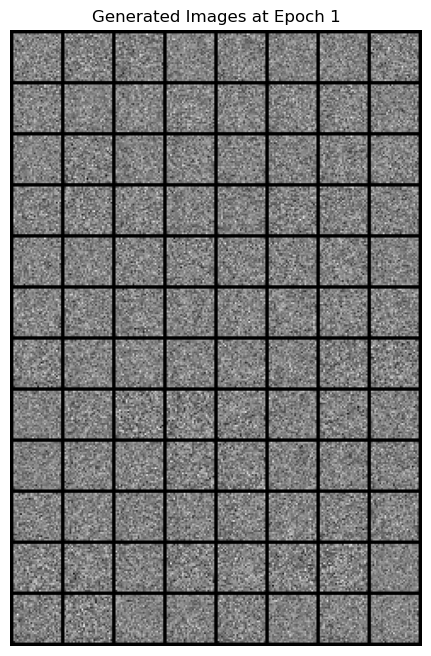
\includegraphics[width=\textwidth]{2-Epoch1.png}
					\caption{epoch 5}
				\end{subfigure}
				\hfill
				\begin{subfigure}[b]{0.3\textwidth}
					\centering
					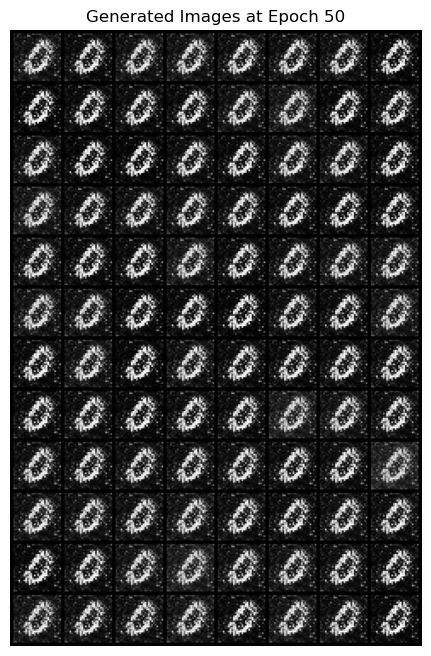
\includegraphics[width=\textwidth]{2-Epoch50.png}
					\caption{epoch 50}
				\end{subfigure}
				\hfill
				\begin{subfigure}[b]{0.3\textwidth}
					\centering
					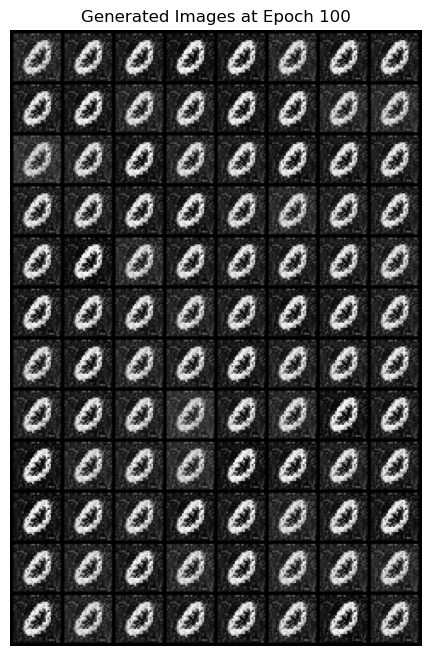
\includegraphics[width=\textwidth]{2-Epoch100.png}
					\caption{epoch 100}
				\end{subfigure}
				\caption{Epochs for GAN (b)}
				\label{epochs_2}
			\end{figure}

		In the comparative analysis of the GAN models, the substitution of Adam with SGD for the generator has led to notably different results.\\
	
		With Adam as the optimizer, the generator consistently produced images that gradually increased in quality and recognizability across epochs. This improvement is likely due to Adam's adaptive learning rate mechanism, which adjusts based on the model's performance.\\
		
		Conversely, when using SGD, the images generated did not exhibit the same level of progression and remained less distinct. This can be attributed to the constant learning rate of SGD, which does not account for the nuanced needs of the generator's training process. The learning curve with SGD also showed greater fluctuations in the generator's loss, indicating challenges in optimizing the model effectively.\\
		
		These observations suggest that the adaptive qualities of Adam are better suited for the intricate dynamics of training GANs, a hypothesis that is supported by the more stable and successful learning trajectory observed when Adam is employed.
		\end{soln}
	
		\item Except the method that we used in (a), how can we improve training for GAN? Implement that and report your setup, learning curves, and generated images in epoch 1, 50, 100.
        This question is an open-ended question and you can choose whichever method you want.
		\hfill (20 pts)
		
		\begin{soln}
			These are the results of executing the third GAN, code attached below.
			\begin{figure}[H]
				\centering
				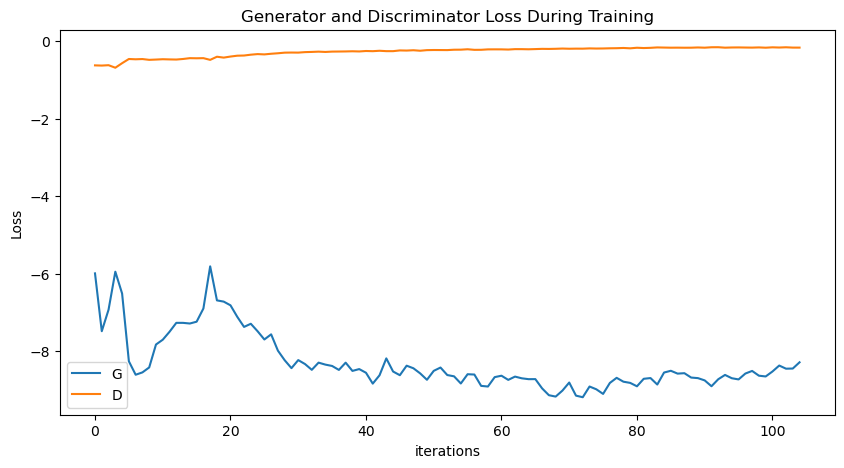
\includegraphics[width=0.7\textwidth]{3-LearningCurve.png}
				\caption{Learning curve for GAN (c)}
				\label{fig:loss_3}
			\end{figure}
			
			\begin{figure}[H]
				\centering
				\begin{subfigure}[b]{0.3\textwidth}
					\centering
					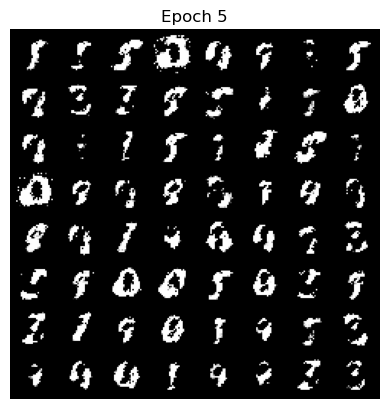
\includegraphics[width=\textwidth]{3-Epoch5.png}
					\caption{epoch 5}
				\end{subfigure}
				\hfill
				\begin{subfigure}[b]{0.3\textwidth}
					\centering
					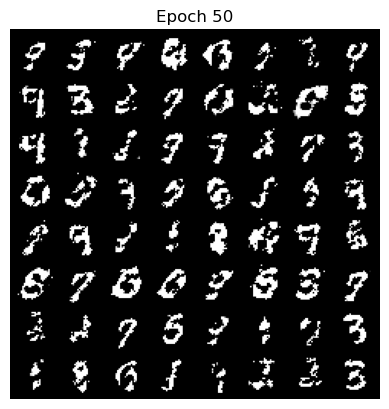
\includegraphics[width=\textwidth]{3-Epoch50.png}
					\caption{epoch 50}
				\end{subfigure}
				\hfill
				\begin{subfigure}[b]{0.3\textwidth}
					\centering
					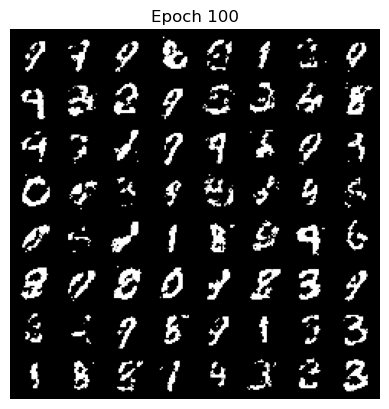
\includegraphics[width=\textwidth]{3-Epoch100.png}
					\caption{epoch 100}
				\end{subfigure}
				\caption{Epochs for GAN (c)}
				\label{epochs_3}
			\end{figure}

			The following improvements were made in the GAN model compared to the first original model:

			\begin{enumerate}
				\item \textbf{Spectral Normalization in Discriminator:} Spectral normalization was applied in the discriminator's layers. This method normalizes the weights, controlling the Lipschitz constant to stabilize the training by preventing the discriminator from overpowering the generator.
			
				\item \textbf{Wasserstein Loss with Gradient Penalty (WGAN-GP):} The model employs the Wasserstein loss function, offering greater stability than Binary Cross Entropy loss. It minimizes an estimate of the Earth Mover's distance between real and generated distributions. The gradient penalty enforces a 1-Lipschitz constraint, enhancing training stability and mitigating mode collapse.
			
				\item \textbf{Differentiated Learning Rates and Adam Optimizer Parameters:} Distinct learning rates and beta parameters for the generator and discriminator optimize each network's training efficiency, addressing the adversarial setup's unique challenges.
			
				\item \textbf{Learning Rate Schedulers:} These schedulers gradually reduce the learning rates during training, aiding in fine-tuning the optimization process for better convergence and stability.
			
				\item \textbf{Noise Addition to Discriminator Inputs:} Adding noise to the discriminator's inputs serves as regularization, preventing overfitting to the training data and improving the diversity of the generated images.
			\end{enumerate}
			
			These enhancements focus on increasing the stability and quality of the GAN training process, addressing common challenges such as training instability and mode collapse, and improving the diversity and realism of the generated images.
		\end{soln}
	
	\end{enumerate}

\section{Directed Graphical Model [25 points]}
Consider the directed graphical model (aka Bayesian network) in Figure~\ref{fig:bn}.
\begin{figure}[H]
    \centering
    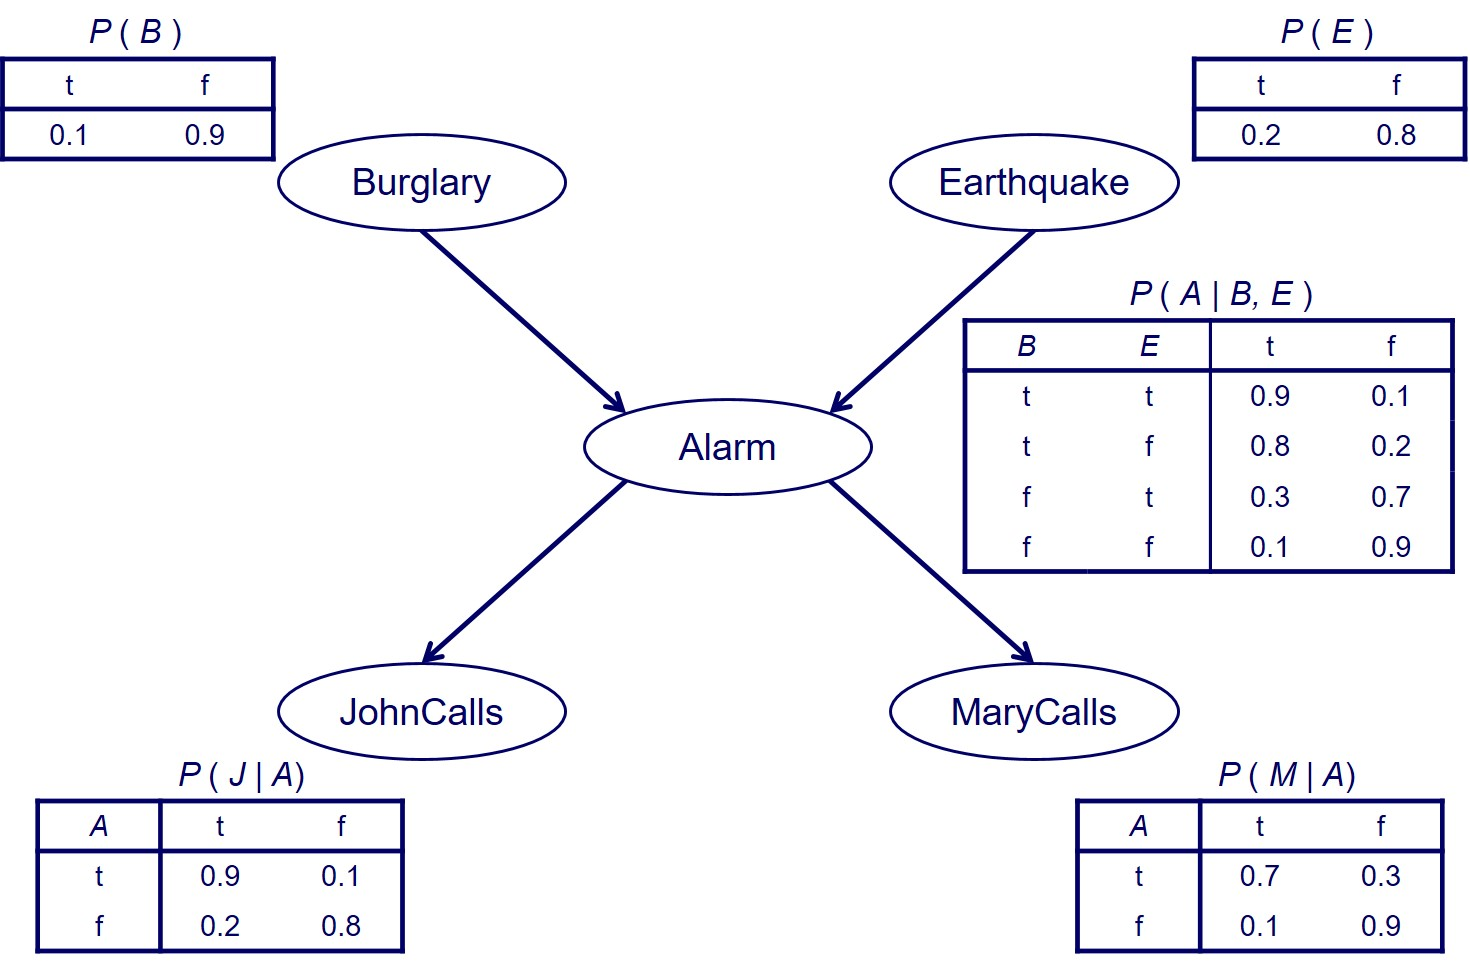
\includegraphics[width=0.8\textwidth]{BN.jpeg}
    \caption{A Bayesian Network example.}
    \label{fig:bn}
\end{figure}
Compute $P(B=t \mid E=f,J=t,M=t)$ and $P(B=t \mid E=t,J=t,M=t)$. (10 points for each) These are the conditional probabilities of a burglar in your house (yikes!) when both of your neighbors John and Mary call you and say they hear an alarm in your house, but without or with an earthquake also going on in that area (what a busy day), respectively.\\

\begin{soln}
    The conditional probabilities can be calculated as follows:

    Given that \( P(B) = 0.1 \), \( P(E) = 0.2 \), and the conditional probability tables for \( P(A | B, E) \), \( P(J | A) \), and \( P(M | A) \), we can calculate:
    \begin{align*}
        P(A = t) =\ & P(B = t, E = t)P(A = t | B = t, E = t) \\
                   & + P(B = t, E = f)P(A = t | B = t, E = f) \\
                   & + P(B = f, E = t)P(A = t | B = f, E = t) \\
                   & + P(B = f, E = f)P(A = t | B = f, E = f)
    \end{align*}    

    After computing \( P(A = t) \), we have \( P(A = f) = 1 - P(A = t) \).

    We can then find \( P(J = t, M = t) \) which is the marginal likelihood of the evidence:

    \[
    P(J = t, M = t) = P(J = t, M = t | A = t)P(A = t) + P(J = t, M = t | A = f)P(A = f)
    \]

    Using Bayes' theorem, the posterior probabilities for \( B \) given \( J \), \( M \), and \( E \) are calculated as:

    \[
    P(B = t | E = f, J = t, M = t) = \frac{P(B = t)P(A = t | B = t, E = f)P(J = t, M = t | A = t)}{P(J = t, M = t)}
    \]

    \[
    P(B = t | E = t, J = t, M = t) = \frac{P(B = t)P(A = t | B = t, E = t)P(J = t, M = t | A = t)}{P(J = t, M = t)}
    \]

    Substituting the values and solving gives us:

    \[
    P(B = t | E = f, J = t, M = t) \approx 0.411
    \]

    \[
    P(B = t | E = t, J = t, M = t) \approx 0.237
    \]

    Thus, the conditional probabilities of a burglary given the evidence of neighbors' calls with and without an earthquake are approximately 41.1\% and 23.7\% respectively.
\end{soln}


\section{Chow-Liu Algorithm [25 pts]}
Suppose we wish to construct a directed graphical model for 3 features $X$, $Y$, and $Z$ using the Chow-Liu algorithm. We are given data from 100 independent experiments where each feature is binary and takes value $T$ or $F$. Below is a table summarizing the observations of the experiment:

\begin{table}[H]
        \centering
                \begin{tabular}{cccc}
                           $X$ & $Y$ & $Z$ & Count \\
                                \hline
                                T & T & T & 36 \\
                                \hline
                                T & T & F & 4 \\
                                \hline
                                T & F & T & 2 \\
                                \hline
                                T & F & F & 8 \\
                                \hline
                                F & T & T & 9 \\
                                \hline
                                F & T & F & 1 \\
                                \hline
                                F & F & T & 8 \\
                                \hline
                                F & F & F & 32 \\
                                \hline
                \end{tabular}
\end{table}

\begin{enumerate}
	\item Compute the mutual information $I(X, Y)$ based on the frequencies observed in the data. (5 pts)
	\item Compute the mutual information $I(X, Z)$ based on the frequencies observed in the data. (5 pts)
	\item Compute the mutual information $I(Z, Y)$ based on the frequencies observed in the data. (5 pts)
	\item Which undirected edges will be selected by the Chow-Liu algorithm as the maximum spanning tree? (5 pts)
	\item Root your tree at node $X$, assign directions to the selected edges. (5 pts)
\end{enumerate}

\begin{soln}
	1. Mutual Information \(I(X, Y)\):
   The mutual information between \(X\) and \(Y\) is calculated using their joint and individual probabilities. The result is:
   \[ I(X, Y) \approx 0.278 \]

2. Mutual Information \(I(X, Z)\):
   Similarly, the mutual information between \(X\) and \(Z\) is computed, yielding:
   \[ I(X, Z) \approx 0.133 \]

3. Mutual Information \(I(Z, Y)\):
   The mutual information between \(Z\) and \(Y\) is the highest among the three pairs, calculated as:
   \[ I(Z, Y) \approx 0.397 \]

4. Maximum Spanning Tree (Edges Selected by the Chow-Liu Algorithm):
   Based on the calculated mutual information, the Chow-Liu algorithm selects the edges with the highest mutual information to form the maximum spanning tree.\\
   The selected edges are:\\
   
   - Edge \(Y-Z\) (highest mutual information)\\
   - Edge \(X-Y\) (second highest mutual information)\\
   
   The edge \(X-Z\) is not selected as it has the lowest mutual information.\\

5. Rooting the Tree at Node \(X\) with Directed Edges:
   After forming the tree, it is rooted at node \(X\), and directions are assigned to the edges. The final directed tree structure is:
   - \(X \rightarrow Y\)
   - \(Y \rightarrow Z\)\\

   This assignment follows from the convention of directing edges away from the root in a directed tree.
\end{soln}

	\bibliography{hw6}
	\bibliographystyle{apalike}
\end{document}
